\documentclass[10pt]{oblivoir}


%-- 논문 주요 정보 표기 
\def\mytitle{Eng Title} % todo: "Eng Title"을 삭제하고 영어 논문 제목을 쓸 것.
\def\mytitleko{우리말 제목} % todo: "우리말 제목"을 삭제하고 우리말 논문 제목을 쓸 것.
 
\def\myauthorfirst{Hong Gildong1} %todo: Hong Gildong1 을 지우고 저자1의 영문 이름을 쓰시오.
\def\myauthorsecond{Hong Gildong2} %todo: Hong Gildong2 을 지우고 저자2의 영문 이름을 쓰시오.

\def\myauthorfirstko{홍길동1} %todo: 홍길동1을 지우고 자신의 이름을 스시오.
\def\myauthorsecondko{홍길동2} %todo: 홍길동2를 지우고 자신의 이름을 스시오. 

\def\affiliation{Sejong Academy of Science and Arts}
\def\affiliationko{세종과학예술영재학교}
\def\address{265, Dalbit 1-ro, Sejong-si, Republic of Korea}

\def\mykeywords{keyword1, keyword2, keyword3} %todo: 키워드 입력 (영문) 
\def\mykeywordsko{주요어1, 주요어2, 주요어3} %todo: 국문 주요어 입력

\def\mydate{2024년\quad 11월\quad OO일} %todo: 제출일 입력
\def\myadvisor{OOO} %todo: 지도교사 이름 입력
%-- 논문 주요 정보 표기 끝

% RnE 양식 구현을 위한 프리엠블 2024.08.21.

\usepackage{fapapersize}
\usefastocksize{210mm,297mm}
\usefapapersize{210mm,297mm,25mm,25mm,25mm,25mm} 
\usepackage{mathtools}
\usepackage{amsthm}
\usepackage{amssymb}
\usepackage{tikz}
\usetikzlibrary{calc,decorations.pathmorphing,shapes,patterns}
\usepackage{rotating}
\usepackage{pgf,pgfplots}
\pgfplotsset{compat=1.15}
\usepackage{mathrsfs}
\usetikzlibrary{arrows}
\usepackage{lipsum}
\usepackage{jiwonlipsum}
\usepackage{tabularray}
\UseTblrLibrary{varwidth,booktabs}
\usepackage{ragged2e}   
\usepackage{textpos}
\usepackage{kskorsymb}

\renewcommand\thesection{\Roman{section}}
\renewcommand\thesubsection{\arabic{subsection}}
\renewcommand\thesubsubsection{\thesubsection.\arabic{subsubsection}}
\setsecnumformat{\csname the#1\endcsname.\ }

%\linespread{1.3} % 영어 논문이므로 줄간격 조절함

\usepackage{caption}

\DeclareCaptionLabelFormat{cjk-single-bracket}{[#1 #2]}
\DeclareCaptionLabelFormat{cjk-angle-bracket}{<#1 #2>}
\captionsetup[figure]{%
labelsep=space,
labelfont=bf,
labelformat=cjk-single-bracket,
name={Fig.}
}
\captionsetup[table]{%
labelsep=period,
labelfont=bf,
%labelformat=cjk-angle-bracket,
name={Table}
}


%%%%%%%%%%%%%%%%%%%%%%%%%%%%%%%%%%%%%%%%%%%%%%%%%%%%%%%%
%-- 정리류 환경 설정
\newtheorem{theorem}{\bfseries\sffamily 정리}%[section]
\newtheorem{lemma}[theorem]{도움정리}
\newtheorem{corollary}[theorem]{따름정리}
\theoremstyle{definition}
\newtheorem{definition}[theorem]{정의}
\newtheorem{example}[theorem]{보기}
\theoremstyle{remark}
\newtheorem{remark}[theorem]{참고}

\numberwithin{equation}{section}
\renewcommand*{\proofname}{증명}
%==
% \renewcommand\qedsymbol{
% \hfill\ensuremath{\blacksquare}
%} 
%====
%-- 정리류 환경 설정 끝

%---- description label 변경
% \renewcommand*\descriptionlabel
% [1]{\hspace\labelsep
% \scshape\mdseries #1}
%---------- description label 변경 끝

\newcommand{\splitatcommas}[1]{%
  \begingroup
  \begingroup\lccode`~=`, \lowercase{\endgroup
    \edef~{\mathchar\the\mathcode`, \penalty0 \noexpand\hspace{0pt plus 1em}}%
  }\mathcode`,="8000 #1%
  \endgroup
}

\newcommand{\mycheckedbox}{$\square $\!\!\!\!\checkmark}




\setcounter{secnumdepth}{3}
\renewcommand{\abstractname}{Abstract} %Abstract 이름 변경

\input{Ltrominoes}
\input{biblatexcontrol.tex} % 참고문헌 표기 방식 설정 파일

\allowdisplaybreaks

%%% RnE 보고서 관련 요약문 등 %%%

%%% 연구결과 요약문 및 과제 수행 과정의 표에 들어가는 내용을 쓰는 곳이다.

%%%--------------------------------------
\newcommand{\summaryGoal}{%%% 연구 필요성 및 목적 쓰는 곳
\jiwon[1] %% todo: 여기의 \jiwon[1]를 삭제하고 "연구의 필요성 및 목적"을 쓸 것 
% "연구 필요성 및 목적 쓰는 곳 끝.
}
%%%---------------------------------------


\newcommand{\summaryResult}{%%% 연구내용 및 연구결과 쓰는 곳
\jiwon[2-3] %% todo: 여기의 \jiwon[2-3]을 삭제하고 "연구내용 및 연구결과"를 쓸 것 
% 연구내용 및 연구결과 쓰는 곳 끝.
}

%%%---------------------------------------
\newcommand{\summaryEffect}{%%% 연구 기대효과 쓰는 곳
\jiwon[4] %% todo: 여기의 \jiwon[4]를 삭제하고 "연구 기대효과"를 쓸 것 
% 연구 기대효과 쓰는 곳 끝.
}

%%%---------------------------------------


\newcommand{\summaryExpert}{%%% 전문가 피드백 활용 과정 쓰는 곳
% 전문가 피드백 활용을 받지 않았다면, 아래 줄의 \jiwon[5]를 삭제하고 "해 당 없 음"이라고 쓴다.
\jiwon[5] %% todo: 전문가 피드백 활용과정에 쓸 내용이 있으면, \jiwon[5]를 지우고 내용을 쓰면 된다.
% 전문가 피드백 활용 과정 쓰는 곳 끝.
}

%%%---------------------------------------


\newcommand{\summaryProblemSolving}{%%% 문제해결 과정 쓰는 곳
\jiwon[6-7] %% todo: 여기의 \jiwon[6-7]을 삭제하고 "문제해결 과정"을 쓸 것 
% 문제해결 과정 쓰는 곳 끝.
}

%%%---------------------------------------
\newcommand{\summaryFirstMember}{%%% 팀원1 내용 쓰는 곳
\jiwon[8] %% todo: 여기의 \jiwon[8]을 삭제하고 "팀원1 "의 내용을 쓸 것 
% 팀원1 내용 쓰는 곳 끝.
}

%%%---------------------------------------

% \newcommand{\summarySecondMember}{%%% 팀원2 내용 쓰는 곳


% % 팀원2 내용 쓰는 곳 끝.
% }


%%%---------------------------------------
\newcommand{\summaryLearning}{%%% 과제 수행 과정에서의 학습 쓰는 곳
\jiwon[9] %% todo: 여기의 \jiwon[9]를 삭제하고 "과제 수행 과정에서의 학습"의 내용을 쓸 것 
% 과제 수행 과정에서의 학습 쓰는 곳
}



\begin{document}
\pagestyle{empty}

\begin{textblock*}{\textwidth}(0cm,0cm)
  \noindent\LARGE\bfseries 1. 연구결과 요약문
\end{textblock*}
\vspace{23pt}
\begin{center}
  \begin{tblr}{
      width = \textwidth,
      colspec = {Q[1,c,m,gray!20]Q[3.88,m]},
      hlines,
      vline{1-Z} = {solid},
      column{1}={font=\bfseries\sffamily}
      }
      과 제 명 & \mytitleko  \\
      {연구 필요성\\ 및 목적} & \summaryGoal \\
      {연구내용 \\ 및 \\ 연구결과} & \summaryResult  \\
      연구 기대효과& \summaryEffect  \\
      {Keyword\\ (5개 이내)}& \mykeywordsko \\
  \end{tblr}    
\end{center}

\newpage

\begin{textblock*}{\textwidth}(0cm,0cm)
  \noindent\LARGE\bfseries 2. 과제 수행 과정
\end{textblock*}
\vspace{23pt}
\begin{center}
  \newlength\mycellwidth
% \setlength\mycellwidth{.76\textwidth}
\setlength\mycellwidth{\dimexpr\linewidth-\parindent-2.5cm-2.5em\relax} % 셀 병합에서 사용한 길이 지정
  \begin{tblr}{
      width=\textwidth,
      measure=vbox,
      colspec = {Q[2.5cm,c,m,gray!20]X[.7,m]X[4.96,m]},
      hlines,
      vline{1-Z} = {solid},
      % cell{1}{2}={c=2}{},
      % cell{2}{1}={r=2}{},
      % cell{2}{2}={c=2}{},
      % cell{Z}{2}={c=2}{},
      column{1}={font=\bfseries\sffamily}
      }
      {전문가 \\ 피드백 활용 \\ 과정} & \SetCell[c=2]{c} {\hsize=\mycellwidth\justifying\summaryExpert\par} &  \\
      \SetCell[r=2]{c,m} {문제해결 \\ 과정} & \SetCell[c=2]{m}  {\hsize=\mycellwidth\justifying\summaryProblemSolving\par}  &  \\
      & \SetCell{l,t} 팀원1 & \summaryFirstMember \\
      % & & \\
      % & & \\
      {과제 수행 \\ 과정에서의 \\ 학습}& \SetCell[c=2]{c} {\hsize=\mycellwidth\justifying\summaryLearning\par}  &   \\
  \end{tblr}        
\end{center}

\newpage


\begin{textblock*}{\textwidth}(0cm,0cm)
  \noindent\LARGE\bfseries 3. 연구결과
  \end{textblock*}
  \vspace{18pt} 
\begin{center}
\begin{spacing}{1.3}
{\LARGE\bfseries    \mytitleko }\par
\vspace{5pt}
\textcolor{gray}{\myauthorfirstko} \par 
\textcolor{gray}{\affiliationko}
\end{spacing}
\vspace{10pt}

{\large\bfseries    \mytitle }\par
\vspace{5pt}
\textcolor{gray}{\myauthorfirst} \par 
\textcolor{gray}{\affiliation}
\end{center} %% 프리엠블 및 본문 시작 제목 표시 설정


\begin{center}{\Large\textbf{국문 초록}} \noindent\rule{\textwidth}{.12mm} \end{center}
%%%%%%%%%%%%%%%%%%%%%%%%%%%%%%%%%%%%%%%%%%%%%%%%%%%%%%%%%%%%%%%%%%%%
%%% 국문 초록 입력 
% 여기에 초록을 입력할 수 있다.
초록은 언제 쓰는가? 맨 나중에 쓰는게 국룰이다. 진짜? 당연하지. 초록은 논문의 얼굴과 같다. 선행연구 \citep{smith1987tiling}에 의하면 어쩌고 저쩌고.


%%%%% 국문 초록 입력 끝
%%%%%%%%%%%%%%%%%%%%%%%%%%%%%%%%%%%%%%%%%%%%%%%%%%%%%%%%%%%%%%%%%%%%
\vskip5pt
\noindent {\bfseries 주제어:}\ \mykeywordsko % 주제어는 메크로 \mykeywordsko 에 의해 자동으로 나타날 것이다. 

\noindent\rule{\textwidth}{.12mm}
 % 초록 내용 


%%%%%%%%%%%%%%%%%%%%%%%%%%%%%%%%%%%%%%%%%%%%%%%%%%%%%%%%%%%%%%%%%%%%
% 이 파일에는 본문 내용을 입력하면 된다.
%%%%%%%%%%%%%%%%%%%%%%%%%%%%%%%%%%%%%%%%%%%%%%%%%%%%%%%%%%%%%%%%%%%%


\section{서론} % 섹션을 시작할 때는  \section{섹션제목} 와 같은 형태로 섹션 제목을 쓰고 그 아래에 본문을 쓰면 된다.

\jiwon[2] % 더미 텍스트

\section{이론적 배경 및 선행연구 조사}\label{sec:search}
\subsection{소제목}
\subsubsection{과학영재 창의연구(R\&E)}

\jiwon[6-7] % 더미 텍스트

앞서 \ref{sec:search}절에서 본 바와 같이 이론적 배경은 매우 어렵다.


\begin{figure}[!ht] % 그림입력
    \centering
    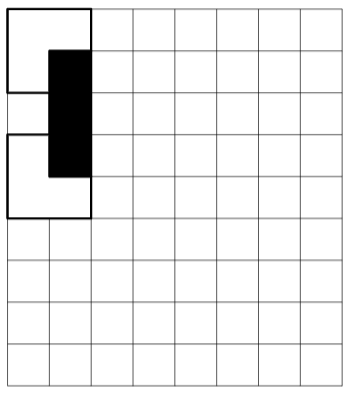
\includegraphics[width=.15\textwidth]{images/B(8, 9).png} % images/그림파일 이름
    \caption{bad pair of $9\times 8$ deficient tile} % 그림 캡션
    \label{fig:my_label} % 그림의 위치를 지시할 때 쓰는 label
\end{figure}

\begin{definition}
정의란 무엇일까? \citep{aanjaneya2009tromino, golomb2021polyominoes, nitica2017tilings} % 참고문헌 표기
\end{definition}

\jiwon[3-4] % 더미 텍스트

\begin{theorem}\label{thm:what}
    정리란 무엇일까?
\end{theorem}



\subsection{그림 삽입 방법}

%--------- 그림 삽입 방법 설명(내용을 확인 한 후에, 삭제하세요).
아래에서는 그림을 삽입하는 방법을 안내한다. 크게 두 가지 방법이 있다.
\begin{enumerate}[(a)]
    \item 그림 파일을 images 폴더에 업로드 한 후, 그 파일을 넣는 방식.
    \item 텍을 이용하여 직접 그림을 그리는 방식.
\end{enumerate}
그러나, 어느 방식이든, 그림의 위치를 \TeX에게 맡기려면, figure 환경을 이용해야한다. 또 하나의 팁을 주자면, 그림파일을 미리 준비하지 않았더라도, \TeX이 갖고 있는 예시그림을 이용하여 그림의 위치를 미리 어느 정도 살펴볼 수 있다는 것이다. 

다음 예시는 \TeX이 갖고 있는 그림예제를 이용하여 그림을 삽입해 본 것이다.

\begin{figure}[!ht]
    \centering
    \includegraphics[width=.4\textwidth]{example-image} % images/그림파일 이름
    \caption{이 그림의 캡션은?!}
    \label{fig:my_fig_label}
\end{figure}


다음 예시는 텍을 이용하여 직접 그림을 그리는 예이다.
\begin{center}
 \begin{tikzpicture}[scale=.5]
 	\checkerboard{15}{15} 	% 그리드를 그리는 명령 \checkerboard{"가로칸 수"}{"세로칸 수"}
	\LtrominoNE{3}{10}
	\LtrominoNW{4}{0}
	\LtrominoSW{6}{1}
	\LtrominoSE{10}{5}
 \end{tikzpicture}
\end{center}
이 그림은 figure 환경에 그린 것이 아니기 때문에, 별도의 캡션이 달려있지는 않다.  figure 환경에 넣은 그림에는 각 그림에 label을 지정해두었으므로, 상호참조 기능을 이용하여 ``그림 \ref{fig:my_label}\을 참고하라.''와 같이 해당 그림을 언급할 수 있다.

한가지 유의할 점은, 논문에서 그림은 필요한 경우에만 넣는 다는 것이다. 다시 말해, 논문에 그림을 넣는 것은 논문의 내용에 (상호참조 등을 통해) 그 그림이 언급하만 가능한 것으로 여기는 것이 일반적이다. 따라서 논문에 등장하는 모든 그림은 figure 환경에 넣는 것이 바람직하다 하겠다.

%------------ 그림 삽입 방법 설명 끝. 

\subsection{표 삽입 방법}
한편 표를 삽입하는 방법은 그림을 삽입하는 방법과 거의 동일하다. figure 환경을 table환경으로 바꾸기만 하면 된다. 표를 텍에서 집접 그리는 것은 좀 번거로울 수 있다. 불편하다면, 다른 표 작성도구로 표를 만든 다음 이를 그림으로 집어 넣되 다만 table 환경을 이용하여 삽입하면 캡션이 자연스럽게 잘 붙을 것이다.

\begin{table}[!ht]
    \centering
    % 표를 만드는 가장 좋은 환경은 tblr 환경이다. (tabularray페키지 필요) 그리고 https://www.tablesgenerator.com/ 를 이용하면 아주 편리하다.
    \caption{이 표의 캡션은?!}
    \label{tab:my_label}
    \begin{tblr}{
    hlines,vlines
    }
          & 위치 & 장소 \\ 
        1 &    &    \\ 
        2 &    &    \\ 
        3 &    &    \\ 
    \end{tblr}
\end{table}

한편 표 \ref{tab:my_booktablabel}에서 볼 수 있는 표 양식은 여러 타이포그라피 교과서에서 권장하는 양식이며, 서구권에서 표준적으로 사용하는 양식이라 할 수 있다.
\begin{table}[!ht]
    \centering
    % 표를 만드는 가장 좋은 환경은 tblr 환경이다. (tabularray페키지 필요) 그리고 https://www.tablesgenerator.com/ 를 이용하면 아주 편리하다.
    \caption{예쁜 표의 캡션은?!}
    \label{tab:my_booktablabel}
\begin{booktabs}{
colspec={cccc}
}
\toprule
Case & Box A & Box B & Remarks \\
\midrule
\SetCell[r=2]{c,m} A & $+X$ & $-1.0$ & \SetCell[r=2]{c,m} B \\
\cmidrule[lr]{2-3}
& $-X$ & $-7.9$ & & \\
\bottomrule
\end{booktabs}
\end{table}


\subsection{수식 입력 방법}
이번에는 수식을 작성하는 몇 가지 예를 살펴보자. 수식은 크게 두 가지 모드로 작성한다.
\begin{itemize}
    \item 행중수식: 문단을 바꾸지 않고 쓰는 수식
    \item 행간수식: 문단을 별도로 두어 별도의 행에 쓰는 수식
\end{itemize}
구체적인 몇 가지 예를 통해서 수식을 입력하는 방법을 살펴보자.

%----------- 수식 작성 예졔
\begin{itemize}
    \item 아래첨자.

아래첨자는, 예를 들어, 이렇게 쓰면 된다. $A_{b+c}$. 여기서 $A_a+b$와 비교해보아라. 아! 그리고 곱하기는 $a\times b$와 같이 쓴다.
\item 최대정수함수 기호. 

국제표준(?) 방식으로 써보자. $\lfloor x\rfloor$로 쓰면 된다. 최대정수함수를 비롯한, 소위, 괄호류(?)는 괄호 안에 들어 있는 수식의 크기에 맞게 괄호의 크기가 바뀌어야겠죠! 아래의 두 식을 비교해 보세요.
\[ \lfloor \frac{\pi^2}{6}\rfloor \]
으, 못생긴 식이다.
\[ \left\lfloor \frac{\pi^2}{6}\right\rfloor \]
그렇다. $\left( \frac{1}{2} \right)$와 같이 쓰면 된다.

\item 분수 표기는 $\frac{2}{3}$과 같이 쓰면 된다. 행간수식을 이용해서 분수를 표기하면 
\[ \frac{df}{dt}=\frac{df}{ds}\frac{ds}{dt} \]
와 같이 분수의 크기가 커진다.


\item 부등호는 알다시피 $1\leq 3\leq 5 \geq 2$.

\item 합동식.

몇 가지 방법이 있다. 우선 세 줄짜리 등호는 $\equiv$ 이렇게. 아래에서는 여러 줄에 걸친 수식을 쓰는 법도 함께 보자. 소스에 등장하는 \& 는 수식을 정렬하는 도구로 이해하면 된다. 줄바꿈은 백슬래시 두 개!
\begin{align*}
a & \equiv b \mod{p} \\
a & \equiv b \pmod{p}
\end{align*}
음, 두 번째 방법으로 쓰면 되겠구나.
\end{itemize}
%---------- 수식 작성 예제 끝.



\section{결론} 
\jiwon[4] % 더미 텍스트



 % 본문 내용

\section{참고문헌}
\printbibliography[heading=none]

%%%% 참고 %%%%
%%\citep{}; 내용에서 참고문헌을 참조할 때는 \citep{aanjaneya2009tromino}와 같이 써서 참조한다.
% 본문에서 참조하지 않지만 참고문헌 목록에 넣고자 할때는 아래와 같이 할 수 있다.
%\nocite{defant2020counting, egge2004132, goodrich2012sorting, park2013avoiding, ulfarsson2011describing}

\newpage
\input{04.appendices.tex}



\end{document}

